\documentclass[tikz, border=5pt]{standalone}
%\usepackage[utf8]{inputenc}
%\usepackage[spanish]{babel}
\usepackage{tikz}
\usetikzlibrary{matrix, backgrounds, arrows, decorations.markings}
\begin{document}
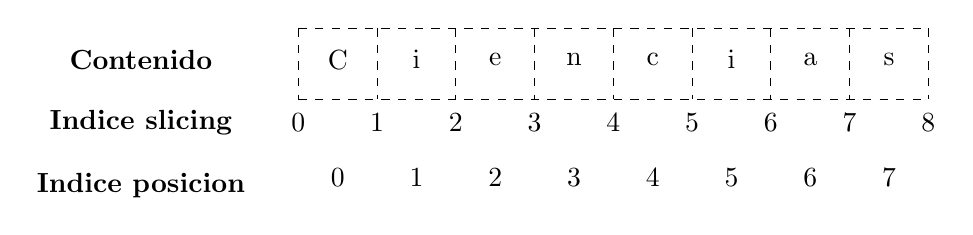
\begin{tikzpicture}
    \node at (0, 0) {$\textbf{Contenido}$};
    \node at (0, -0.8) {$\textbf{Indice slicing}$};
    \node at (0, -1.6) {$\textbf{Indice posicion}$};
    \draw [dashed] (2, 0.4) -- (10, 0.4);
    \foreach \x in {2, ..., 10}
        \draw [dashed] (\x, 0.4) -- (\x, -0.5);
    \draw [dashed] (2, -0.5) -- (10, -0.5);

    \node at (2.5, 0) {C};
    \node at (3.5, 0) {i};
    \node at (4.5, 0) {e};
    \node at (5.5, 0) {n};
    \node at (6.5, 0) {c};
    \node at (7.5, 0) {i};
    \node at (8.5, 0) {a};
    \node at (9.5, 0) {s};

    \node at (2, -0.8) {$0$};
    \node at (3, -0.8) {$1$};
    \node at (4, -0.8) {$2$};
    \node at (5, -0.8) {$3$};
    \node at (6, -0.8) {$4$};
    \node at (7, -0.8) {$5$};
    \node at (8, -0.8) {$6$};
    \node at (9, -0.8) {$7$};
    \node at (10, -0.8) {$8$};
    
    \node at (2.5, -1.5) {$0$};
    \node at (3.5, -1.5) {$1$};
    \node at (4.5, -1.5) {$2$};
    \node at (5.5, -1.5) {$3$};
    \node at (6.5, -1.5) {$4$};
    \node at (7.5, -1.5) {$5$};
    \node at (8.5, -1.5) {$6$};
    \node at (9.5, -1.5) {$7$};

\end{tikzpicture}
\end{document}